%%%%%%%%%%%%%%%%%%%%%%%%%%%%%%%%%%%%%
% Stylish Article
% LaTeX Template
% Version 2.0 (13/4/14)
%
% This template has been downloaded from:
% http://www.LaTeXTemplates.com
%
% Original author:
% Mathias Legrand (legrand.mathias@gmail.com)
%
% License:
% CC BY-NC-SA 3.0 (http://creativecommons.org/licenses/by-nc-sa/3.0/)
%
%%%%%%%%%%%%%%%%%%%%%%%%%%%%%%%%%%%%%%%%%

%----------------------------------------------------------------------------------------
%	PACKAGES AND OTHER DOCUMENT CONFIGURATIONS
%----------------------------------------------------------------------------------------

\documentclass[fleqn,10pt]{SelfArx} % Document font size and equations flushed left
\usepackage[spanish]{babel}
\usepackage{booktabs}
\usepackage{array}


%----------------------------------------------------------------------------------------
%	COLUMNS
%----------------------------------------------------------------------------------------

\setlength{\columnsep}{0.55cm} % Distance between the two columns of text
\setlength{\fboxrule}{0.75pt} % Width of the border around the abstract

%----------------------------------------------------------------------------------------
%	COLORS
%----------------------------------------------------------------------------------------

\definecolor{color1}{RGB}{0,0,90} % Color of the article title and sections
\definecolor{color2}{RGB}{0,20,20} % Color of the boxes behind the abstract and headings

%----------------------------------------------------------------------------------------
%	HYPERLINKS
%----------------------------------------------------------------------------------------

\usepackage{hyperref} % Required for hyperlinks
\usepackage{cite}
\hypersetup{hidelinks,colorlinks,breaklinks=true,urlcolor=color2,citecolor=color1,linkcolor=color1,bookmarksopen=false,pdftitle={Title},pdfauthor={Author}}
\setlength{\extrarowheight}{1.5pt}

%----------------------------------------------------------------------------------------
%	ARTICLE INFORMATION
%----------------------------------------------------------------------------------------

\JournalInfo{Taller de Biotecnología Animal, 2014-I} % Journal information
\Archive{miniReview} % Additional notes (e.g. copyright, DOI, review/research article)

\PaperTitle{Transfección en Animales} % Article title

\Authors{Juan Manuel Iglesias Artola\textsuperscript{1}, Gianfranco Villamonte Cuneo\textsuperscript{1}} % Authors
\affiliation{\textsuperscript{1}\textit{Facultad de Ciencias Biológicas, Universidad Ricardo Palma, Lima, Peru}} % Author affiliation
%\affiliation{\textsuperscript{2}\textit{Department of Chemistry, University of Examples, London, United Kingdom}} % Author affiliation
\affiliation{*\textbf{Correspondencia}: jmanuel9112@icloud.com / giancuneo@gmail.com } % Corresponding author


%----------------------------------------------------------------------------------------
%	ABSTRACT
%----------------------------------------------------------------------------------------

\Abstract{La transfección es el proceso de introducir nucleótidos en una célula, cuyo producto es la transgénesis. Existen múltiples métodos biológicos , físicos y químicos que permiten realizar esta introducción de nucleótidos. Además de la aparicion de múltiples métodos nuevos de transfección en los últimos años, su eficiencia se sigue incrementando. Esto ha permitido la aparición sin precedentes de un sinnúmero de aplicaciones (biomédicas, alimenticias, etc.) que plantean nuevos debates éticos y generan la necesidad de modernizar la reglamentación relacionada.  }


\Keywords{transfección --- transgénicos --- bioética} % Keywords - if you don't want any simply remove all the text between the curly brackets
\newcommand{\keywordname}{Palabras clave} % Defines the keywords heading name

%----------------------------------------------------------------------------------------

\begin{document}

\flushbottom % Makes all text pages the same height

\maketitle % Print the title and abstract box

\tableofcontents % Print the contents section

\thispagestyle{empty} % Removes page numbering from the first page

%----------------------------------------------------------------------------------------
%	ARTICLE CONTENTS
%----------------------------------------------------------------------------------------

\section{Introducción} 

La transfección ha permitido  expresar genes de interés en células eucariotas. Esta capacidad ha posibilitado obtener un mejor entendimiento de la biología celular, la biología molecular y la genética de las células. Al expresar proteínas en células de animales, se ha podido entender aspectos detallados de la síntesis protéica,  los efectos de las mutaciones en su función en las proteínsa, las interacciones entre estas y las interacciones intercelulares. Además, esta tecnología ha llevado al desarrollo de animales trangénicos, a la fertilización \textit{in vitro}, y a la posibilidad de usar la tranferencia de genes para tratar desórdenes genéticos.

Los virus fueron por mucho tiempo la forma más conveniente de transferir genes a células mamíferas. En 1973 Graham y van der Eb \cite{Graham:1973aa} utilizaron el adenovirus 2 para transfomar células de rata, mientras que en 1984 Cepko et al. \cite{Cepko:1984aa} desarrollaron un retrovirus murínico para la introducción de secuencias de DNA en células mamíferas. Si bien los virus constituyen un medio eficiente para lograr la transfección \textit{in vitro}, la construcción de los vectores es laboriosa, consume tiempo, y tiene diversas limitaciones para su uso \textit{in vivo}.

Si bien la transfección por medio de vectores virales es altamente eficiente, otros métodos han sido desarrollados. Los trabajos realizados por Pagano et al. \cite{Pagano:1967aa} fueron pioneros en su área al lograr una alta transferencia de genes a células mamíferas utilizando dietilaminoetil-dextrano (DEAE-D) mezclado con RNA y DNA  \cite{McCutchan:1968aa, Pagano:1967aa}. Después, se demostró que otros métodos también son eficaces: la encapsulación de DNA utilizando liposomas \cite{Fraley:1980aa, Wong:1980aa, Straubinger:1983aa, Fraley:1981aa}, la fusión inducida por polietilenglicol del DNA en los eritrocitos fantasma \cite{Straus:1980aa}, la electroporación \cite{Neumann:1982aa}, los coprecipitados de fosfato de calcio/DNA \cite{Wigler:1979aa}, y los policationes/dimetil sulfóxidos \cite{Kawai:1984aa}. No existe un método indicado para todo tipo celular; sino, la eficiencia de los métodos utilizados varía con respecto a estos y en general, no fueron muy eficientes y presentaban una alta toxicidad celular.

En la actualidad existen tres grandes grupos de métodos que pueden ser utilizados \cite{Kim:2010aa}: \textit{a)} los métodos biológicos, \textit{b)} los métodos químicos y \textit{c)} los métodos físicos. En este minireview se resumen las estrategias experimentales más generales, sus aplicaciones y las implicaciones bioéticas que puede tener la transfección de células animales.

%================Cuadro 1 ==============================
\begin{table*}[th!]
\centering
\begin{tabular}{p{8cm} p{4cm}} \toprule
\textbf{Gen} & \textbf{Detección} \\ \hline
$\beta$-galactosidasa ($\beta$-gal) & Enzimático y colorimétrico \\ 
Cloranfenicol acetil transferasa (CAT) & Enzimático y radioactivo \\
Luciferasa & Luminiscencia \\
Proteína verde fluorescente (GFP) & Fluorescencia \\ \bottomrule
\end{tabular}
\caption{Genes reporteros comunes}
\label{Tab:reportero}
\end{table*}
%================Cuadro 1 ==============================

\section{Métodos de Transfección}
Se han desarrollado diversas técnicas de transfección que cumplen con el propósito de transferir ácidos nucléicos al interior de las células. Existen ciertas características que permiten una transfección exitosa, estas son: alta eficiencia en el transporte del ácido nucléico a la ubicación celular apropiada (el núcleo para el DNA plasmídico y el citoplasma para el RNA); baja toxicidad celular; mínima interferencia con la fisiología celular normal; uso sencillo y reproducibilidad \cite{Schenborn}. Para el caso de la transfección génica utilizada para terapias se deben tomar consideraciones adicionales tales como la vida-media y el transporte a un tipo de célula específica. También se debe decidir si se desea una transfección estable o transitoria.  En esta sección se discuten los tres principales métodos de transfección: los métodos biológicos, químicos y físicos.

\subsection{Transfección transitoria}
La transfección transitoria de genes esta sujeta a varios parámetros. El método de transfección, la fisiología celular y el tipo celular (cultivos en suspensión o adherentes), el método enzimático o colorimétrico utilizado para cuantificar la actividad del gen reportero, la cantidad de DNA y la normalización de la data. El periodo de expresión del gen en una transfección génica varía entre 24 a 72 h y para el éxito del procedimiento son críticas las condiciones celulares, con las  células saludables y las que se encuentren en división las más susceptibles a aceptar plásmidos recombinantes. Par determinar la efeciencia y reproducibilidad de la transfección se puede utilizar un segundo gen reportero que exprese un producto génico que pueda ser detectado y medido de manera sencilla. Tal gen reportero no debe estar presente en el genoma del tipo celular o, en el peor de los casos, puede estar presente pero debe ser expresado en bajos niveles. Los genes reporteros más utilizados se presentan en el Cuadro \ref{Tab:reportero}.

Es importante recalcar que la eficiencia en la expresión del gen reportero disminuye drásticamente con la  integridad del plásmido y su habilidad por llegar al núcleo \cite{Zohar:2001aa}. 

Los métodos de transfección transitoria generalmente dirigen el DNA plasmídico al citoplasma y no está claro qué porcentaje de estas moléculas lineares o circulares alcanzan el núcleo celular. Además, los parámetros experimentales deben ser definidos con cuidado para lograr cierto grado de reproducibilidad. Se ha sugerido que entre los diferentes mecanismos, la difusión pasiva de los plásmidos a través del citoplasma y los poros nucleares representa la forma más probable por la cual los genes reporteros  pueden migrar al núcleo celular y ser activados transcripcionalmente.  Sin embargo, existe evidencia que sugiere otro mecanismo para explicar la transferencia del DNA plasmídico al núcleo celular basado en las señales de importanción del DNA \cite{Vacik:1999aa, Zohar:2001aa}. Se piensa que existe una interacción proteína-DNA plasmídico en el citoplasma y que tales interacciones con factores de transcripción producen señales de localización nuclear, permitiendo la importación de DNA exógeno al núcleo.

\begin{figure*}[ht]
\centering
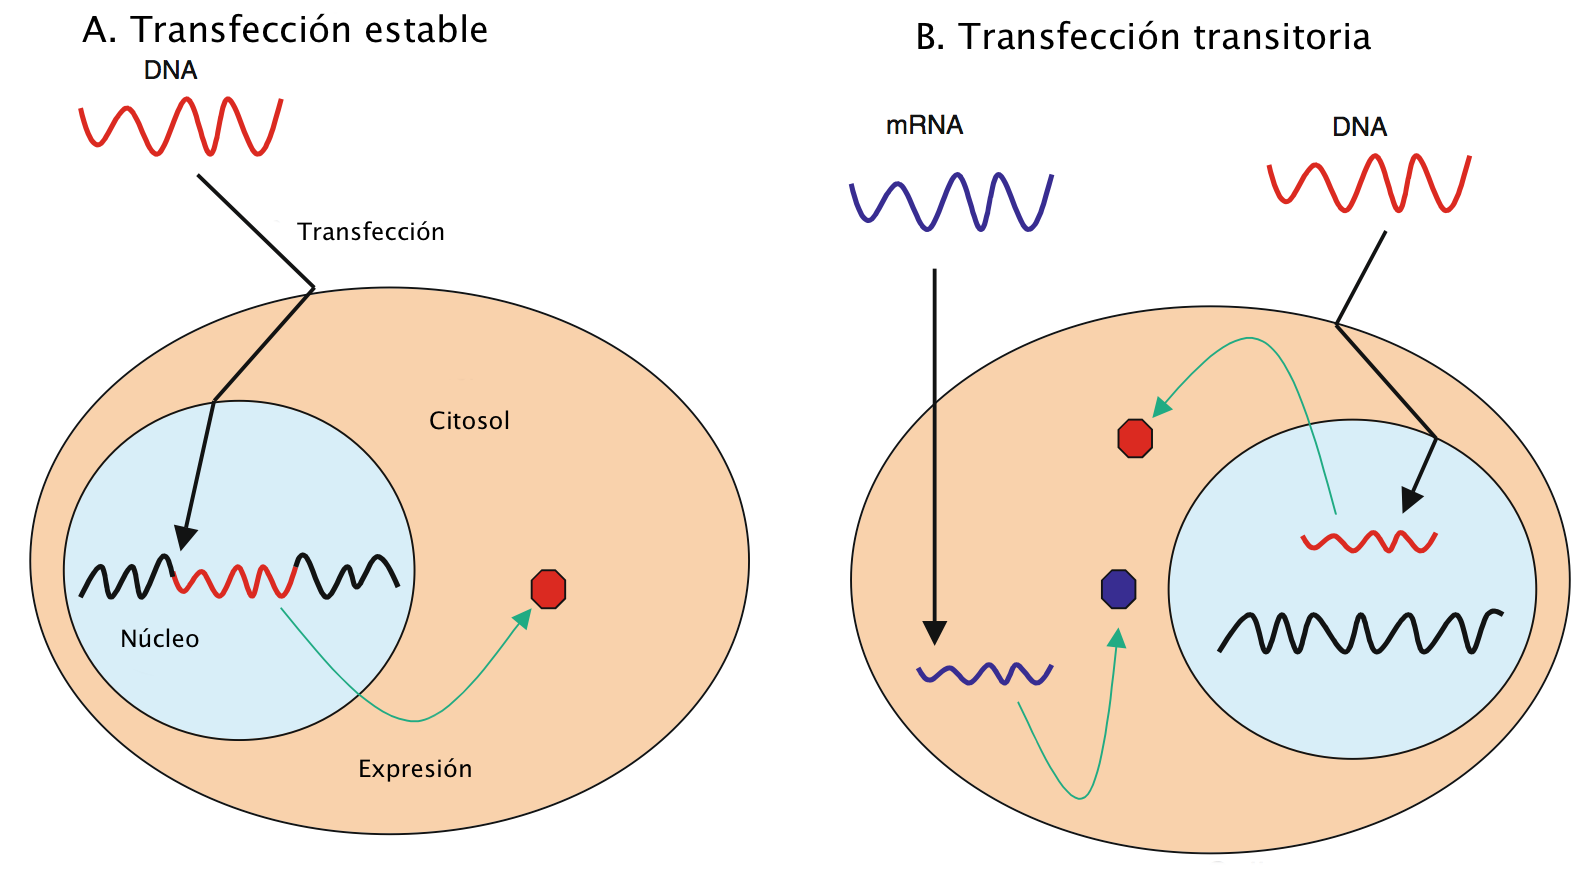
\includegraphics[width=0.8\linewidth]{images/transfeccion.png}
\caption{Diagrama esquemático de dos transfecciones diferentes. A. Transfección estable. El DNA foráneo (rojo) es llevado al núcleo al pasar por la membrana celular y nuclear. El DNA es integrado al DNA genómico (negro) y expresado de manera sostenible. B. Transfección transitoria. El DNA foráneo es transportado dentro del núcleo pero no es integrado en el genoma. El mRNA (azul) también es llevado al citosol, en donde es traducido. Los hexágonos representan las proteínas expresadas a partir de los ácidos nucléicos transfectados. Las flechas negran muestran el transporte del ácido nucléico. Tomado de \cite{Recillas}}
\label{Fig:transfeccion}
\end{figure*}

\subsubsection{Métodos biológicos}La eficiencia de la transfección en esta caso depende de factores como la proporción ácido nucléico/químico, pH de la solución y las condiciones de la membrana celular, todo esto lleva a que el proceso de transfección tenga una baja eficiencia, especialmente \textit{in vivo}, comparado con los métodos mediados por virus. Sin embargo, estos métodos presentan baja citotoxicidad, no existe mutagénesis, no hay DNA extra y no tiene límites de tamaño para el ácido nucléico. Se debe tomar en cuenta que la eficiencia de la transfección química varía dependiendo del tipo de célula a utilizar.

\paragraph*{Coprecipitación con fosfato de calcio}
En este método el calcio de asocia con las cargas negativas del ácido nucléico. La adición de un buffer fosfato resulta en la precipitación del DNA con el calcio y el fosfato, formando pequeñas partícular.  Lo que posibilita que el DNA pueda ingresar a las células por fagocitosis \cite{Loyter:1982aa}. Para que la trasfección sea satisfactoria se debe controlar el tamaño del precipitado; puesto que, se ha correlacionado los precipitados pequeños con una mayor eficiencia de transfección \cite{Jordan:1996aa}. Para esto se debe tomar en consideración que el tamaño de las partículas es sensible a la concentración de calcio y DNA, el pH, la temperatura y el modo en el que el buffer salino y la solución de DNA son mezclados durante la precipitación. Para lograr una alta concentración de DNA, se puede incluir un plásmido inerte p DNA genómico de alto peso molecular \cite{Strain:1985aa}.

\paragraph*{DEAE-Dextrano}
Dietilaminoetildextrano, or DEAE-dextrano, es un reactivo polimérico policatiónico que se une a y transfecta ácidos nucléicos \cite{McCutchan:1968aa}.  El complejo DEAE-dextrano/DNA puede ser tomado por la célula por endocitosis o fagocitosis \cite{Yang:1997aa, Luthman:1983aa}. Se ha encontrado que el tratamiento con cloroquina incrementa la expresión del DNA transfectado en algunos tipos celulares, posiblemente al neutralizar el pH de los lisosomas en los cuales el DNA es internalizado \cite{Luthman:1983aa}. Es necesario que durante el proceso de transfección la morfología celular sea monitoreada puesto que el DEAE-dextran puede ser altamente tóxico para las células.

\paragraph*{Liposomas catiónicos}
El primer lípido catiónico sintético publicado como un transportador de ácidos nucléicos fue el bromuro de 1,2-dioleiloxipropil-3-trimetilamonio (DOTMA) desarrollado por Felgner el al \cite{Felgner01111987}. Desde entonces se han diseñad diferentes tipos de lípidos catióonicos sintéticos para la transfección, conservando la misma estructura general del DOTMA, con un grupo mono o policationico covalentemente adherido a una porción lipofílica. La región catiónica de la molécula se asocia con las cargas negativas de los ácidos nucléicos. Se ha correlacionado una carga total positiva o neutra del complejo lípido/DNA con una mayor eficiencia de transfección de células in vitro. Se piensa que la carga positiva o neutra reduce la repulsión electrostática entre el ácido nucléico y la membrana celular cargada negativamente. Se piensa, también, que el complejo lípido/DNA ingresa a la célula por endocitosis.  Se puede liberar el ácido nucléico de las vesículas endosomales utilizando otros lípidos, tales como dioleilfosfatidiletanolamina (DOPE) en la formulación del liposoma \cite{Farhood:1995aa}. 

Existen tres parámetros esenciales que necesitan ser optimizados para poder utilizar cualquier liposoma en la transfección. Cada tipo celular requiere que se determine una cantidad óptima de DNA en combinación con la concentración del lípido catiónico. Existe una concentración óptima de DNA y lípido para cada tipo celular, con una alta toxicidad en concentraciones elevadas y baja eficiencia en bajas concentraciones. Otro parámetro que requiere optimización es el intervalo de tiempo de la transfección, dependiendo de los reactivos y las condiciones utilizadas, el intervalo de tiempo puede variar entre 1 a 24 horas. Las incubaciones más largas son por lo general más tóxicas.

\subsubsection{Métodos físicos}
Los métodos de tranfección físicos se han desarrollado recientemente y utilizan una diversa gama de herramientas físicas para transportar los ácidos nucléicos al interior de las células. Estos métodos incluyen la microinyección directa, el transporte balístico de partículas, la electroporación, y la transfección basada en láseres \cite{Mehier-Humbert:2005aa}.  

\paragraph*{Microinyección}
En general, el método de micro inyección introduce de manera directa el ácido nucléico en el citoplasma o núcleo \cite{Martinou:1995aa, Ikeda:1995aa}. Este método es efectivo en la introducción de los ácidos nucléicos dentro de las células pero requiere de mucha habilidad, bastante tiempo y ocasionalmente ocasiona la muerte celular. 

Esta técnica ha sido aplicada exitosamente para transferir genes a células musculares y particularmente a células epiteliales \cite{Sawamura:2002aa, Davis:1993aa}. Una limitación de este procedimiento es la falta de control de parámetros como la concentración de DNA plasmídico, la degradación y la eficiencia en la transferencia de genes. Sin embargo para aplicaciones específicas como la transferencia ectópica de genes, este procedimiento tiene ventajas sobre los otros métodos.

\paragraph*{Métodos balísticos}
El transporte de partículas por medios balísticos emplea partículas de oro que se conjugan con los ácidos nucléicos \cite{Lo:1994aa, OBrien:2006aa}. Estos conjugados son disparados a alta velocidad dentro de las células receptoras (``pistola de genes''). Dentro de la célula el ácido nucléico se disocia de las partículas de oro.  Este método es sencillo y confiable pero requiere de equipos y causa daños físicos a las muestras. 

Se han diseñado diferentes tipos de intrumentos para este método. Las ácidos nucléicos son primero precipitados en esferas de oro y depositas en hojas de Mylar. Las partículas de DNA/oro o RNA/oro son colocadas en el instrumento para después ser aceleradas por una descarga de alto voltaje y lanzadas a las células o tejidos de elección. Los dispositivos comerciales utilizan un pulso de helio a baja presión para acelerar las esferas de oro. Con estos dispositivos, las muestras pueden ser preparadas utilizando tubos recubiertos con partículas de oro. 

\paragraph*{Electroporación}
La electroporación es el método físico más empleado; sin embargo, se desconoce el mecanismo exacto, pero se supone que los pulsos eléctricos perturban las membranas celulares, produciendo agujeros por los cuales los ácidos nucléicos pueden ingresar \cite{Inoue:2001aa}. Debido a que la electroporación es un método sencillo y rápido, es posible tranfectar un gran número de células en poco tiempo una vez que se han determinado las condiciones óptimas para la electroporación.  Las células son suspendidas en una concentración de 10$^6$-10$^7$ células/mL en un buffer salino de electroporación, buffer salino HEPES o medio de cultivo sin suero (las células adherentes necesitan ser tripsinizadas antes de la electroporación). Las células son después transferidas a una cubeta estéril y se añade el DNA a ser transferido. Para los experimentos en los que se necesita una expresión transitoria, se añade DNA superenrrollado a una concentración de 10-40 $\mu$g/mL; para una transfección estable se añade DNA lineal con una concentración de 1-20 $\mu$g/mL.  Después de mezclar las células con el DNA para la transfección, son sometidas a uno o más electroshocks, las células son incubadas en medio selectivo después de un periodo de recuperación. 

Los parámetros más críticos a optimizar para cualquier tipo celular son la magnitud del voltaje y la duración del pulso de corriente. Para esto, son efectivas las combinaciones de voltajes altos con pulsos de corto tiempo o voltajes bajos con tiempos más largos. Sin embargo, las condiciones óptimas dependen de las características de la célula, conjuntamente con la conductividad del buffer de electroporación y la temperatura. La electroporación puede realizarse a temperatura ambiente o en hielo, pero es necesario determinar empíricamente las condiciones óptimas para cada tipo célula \cite{Chu11021987}.  El voltaje excesivo y/o la duración de los pulsos resulta en la muerte celular. Durante el establecimiento de las condiciones adecuadas  de electroporación se debe monitorear el ratio entre muerte celular y eficiencia de transferencia para un tipo celular dado. La transfección óptima debe ocurrir bajo condiciones que  causen aproximadamente el 50\% de muerte celular \cite{Schenborn}.

\paragraph*{Láser}
La transfección mediada por láser (también conocida como optoporación o fototransfección) utiliza un pulso de láser para irradiar la membrana celular con la finalidad de formar un poro momentáneo \cite{Shirahata:2001aa, Barrett:2006aa}. Cuando el láser induce la formación del poro, los ácidos nucléicos en el medio son trasferidos dentro de la célula debido a la diferencia osmótica entre el medio y el citosol. El método de láser permite observar a la células siendo transfectada y hacer poros en cualquier ubicación de la célula. Este método puede ser aplicado a células pequeñas, debido a que utiliza un láser, pero para tal caso es necesario un sistema de microscopio láser. 

Además de los métodos mencionados, existen otros métodos físicos como el ultrasonido (sonoporación) y la utilización de un campo magnético (magnetofección) \cite{Kim:1996aa, Dobson:2006aa, Scherer:2002aa}

\subsection{Transfección estable}
Para la generación de líneas celulares estables el transgen de interés debe ser cotransfectado con un marcador de selección que produzca resistencia a una droga. Para cada ensayo de transfección estable se debe monitorear de manera cuidadosa la integración del transgen en el genoma de la célula blanco. En un experimento de transfección típico se debe permitir a las células recuperarse de la transfección por un periodo de 24 a 72 horas en la ausencia de selección. Esto permite a la célula expresar la cantidad necesaria de la enzima de resistencia para proteger a las células transfectadas establemente contra la droga. Después de 48 o 72 horas de la transfección el medio de cultivo debe ser vambiado y reemplazado con medio nuevo complementado con la droga. La selección se produce dentro de las primera a las tercera semana posterior a la transfección con cambios frecuenctes del medio de cultivo selectivo. Finalmente la integridad y número de copias del gen debe ser determinado por Southern blot. 

El método más utilizado en la investigación clinical para lograr una transfección estable es el de la transfección mediada por virus, también conocida como transducción \cite{Pfeifer:2001aa}. Este método es altamente eficiente debido a la naturaleza viral de la integración en el genoma del huésped. Por ejemplo, se ha utilizado el virus de la leucemia murina (MLV)  como vector viral para establecer la expresión sostenible de genes de interés en humanos \cite{Hacein-Bey-Abina:2002aa, Roesler:2002aa}. El MLV integra su DNA en el genoma del hospedero, el cual es posteriormente expresado. El DNA del MLV integrado se replica con el genoma del hospedero, lo que permite la expresión sostenible del gen de interés.

La citotoxicidad y la inmunogenicidad representan las mayores desventajas de la transfección mediada por virus. La introducción del vector viral puede causar una reacción inflamatoria y una mutación insercional, debido a que ciertos vectores virales se integran de manera azarosa al genoma del hospedero, lo cual puede afectar a genes supresores de tumores, activar oncogenes, o interrumpir genes esenciales \cite{Woods:2003aa}. Otra desventaja de este método es que la cápside de un virus tiene espacio limitado para que un gen extraño continúe siendo infectivo. 

\section{Aplicaciones de la Transfección}

La transfección es una herramienta para la modificación genética. Gracias a sus múltiples métodos es posible realizar innumerables aplicaciones como:
\begin{itemize}[noitemsep] % [noitemsep] removes whitespace between the items for a compact look
\item \textbf{Estudios Genéticos}: Genes 'knockout' o 'knockdown' para estudiar su expresión fenotípica.
\item \textbf{Terapia Génica}: Cura de enfermedades.
\item \textbf{Proteínas Recombinantes}: Uso de animales como 'bio-fábricas'.
\item \textbf{Alimentos Transgénicos}: Modificaciones genéticas principalmente para alimentación.
\item \textbf{Mascotas transgénicas}: Peces brillantes, gatos hipoalergénicos, etc.
\end{itemize}

\subsection{Estudios Genéticos}

La transfección puede ser útil para el estudio del funcionamiento de genes. Esto se puede realizar por varios medios: introduciendo un gen de otro organismo (transgenésis), mediante un knockout o knockdown que anule la expresión de un gen \cite{cryanin2004}, aumentando la expresión del gen de estudio \cite{yanni2004laboratory}, o alterando la estructura de la proteína que codifica \cite{ripps1995transgenic}.

De esta manera, este procedimiento ha permitido la realización de estudios sobre el funcionamiento de diversos genes humanos, principalmente con fines médicos.

Estas investigaciones incluyen el análisis de la influencia genética en trastornos psicológicos y neurodegenerativos, mediante la evaluación del fenotipo producido utilizando mecanismos de transfección (principalmente utilizando modelos murinos). Así vemos que la transfección ha permitido evaluar el impacto de la reducción de la enzima SOD-1 en la neurodegeneración producida en la Esclerosis Lateral Amiotrófica (ELA) \cite{ripps1995transgenic}. Asimismo, ha permitido el estudio de la relación de diversos receptores de neurotransmisores con la depresión \cite{cryanin2004}, el autismo, la esquizofrenia, el Alzheimer, la enfermedad de Huntington, entre otros \cite{anthe2002}.

La transfección también ha permitido evaluar el impacto de los genes en la regulación enzimática del metabolismo de lipidos, relacionada con enfermedades cardio-vasculares como la aterosclerosis\cite{yanni2004laboratory}


\subsection{Terapia Génica}

La terapia génica es una importante aplicación de la transfección a la medicina. Muchos de sus usos continuan en experimentación \textit{'in vitro'} o en animales, sin embargo, este campo tiene un gran potencial:
\begin{itemize}[noitemsep] % [noitemsep] removes whitespace between the items for a compact look
\item \ Cáncer
\item \ Enfermedades congénitas
\item \ Curación de heridas , quemaduras y otras afecciones epiteliales
\end{itemize}

La terapia génica se puede emplear para curar diversos tipos de cáncer mediante múltiples métodos. Uno de estos métodos es el de 'vacunación' anti-tumoral. Este consiste en utilizar la transfección para producir antígenos asociados al crecimiento tumoral. Además, se puede utilizar esta tecnología para inducir la producción de citoquinas que inhiban la angiogénesis. Asimismo, se puede usar para inducir el metabolismo de protoxinas por las células tumorales, haciendo que los medicamentos contra el cáncer sean de un impacto más directo y controlado\cite{Vile, Seung}.

La terapia génica puede asimismo ser utilizada para suprimir o controlar enfermedades congénitas, o aliviar sus síntomas, evitando a su vez los efectos secundarios que podría producir el uso de fármacos \cite{Spink}

En el caso de quemaduras, cortes, o afecciones epiteliales provocadas por diversas enfermedades (como el acné o el lupus eritematoso), muchas veces, la curación es lenta y deja muchas cicatrices debido a la ausencia o a la baja producción de factores de crecimiento. La transfección en tejidos epiteliales, probada a la fecha sólo en cultivos celulares y ratones, ha comprobado ser útil tanto para fomentar la regeneración de dichos tejidos, como para inducir su vascularización y reducir las cicatrices \cite{branskigene2006, Reinhart, strulovicihuman2007}.

\subsection{Proteínas Recombinantes}

Uno de los principales objetivos de la modificación genética de animales es la producción masiva de proteínas. Al buscarse en estos casos la producción, en lugar de la expresión en el animal en sí, la modificación genética en estos casos se enfoca en la leche de diversos mamíferos(ovejas, cabras, vacas, chanchos, entre otros).  Esta producción masiva se concentra en proteínas humanas de aplicación biomédica como algunos factores de coagulación, fibrinógeno, colágeno, enzimas y anticuerpos de origen humano; además de en la producción de proteínas de origen viral que podrían servir para inmunizar a las personas ante diversas enfermedades(ver cuadro\ref{cuadro1})\cite{Durocher15012002, Koszarycz2004, niemann2007transgenic, houdebine2009production}. 


\begin{table*}[t!]
\centering
\begin{tabular}{l l l} \toprule
\textbf{Proteína} & \textbf{Enfermedad / Objetivo} & \textbf{Animal} \\ \hline
Activador Tisular del Plasminógeno (t-PA) &Trombosis & Cabra, ratón \\ 
Anti-CD137 & Enfermedades autoinmunes & Cabra \\ 
Albúmina de suero humano (HSA) & Mantenimiento de volumen sanguíneo & Ratón, vaca \\
$\alpha$-lacta albúmina & Anti-infección & Vaca \\
$\alpha$-1 antitripsina ($\alpha$-AT) & Deficiencia lleva a enfisema & Oveja \\
$\alpha$-glucosidasa & Enfermedad de Pompe & Conejo \\
Antitrombina 3 (ATIII) & Trombosis & Cabra \\
CFTR & Fibrosis Quística & Oveja , ratón \\ 
Calcitonina humana & Osteoporosis & Conejo \\ 
Colágeno I & Reparación de Tejidos & Vaca \\ 
Colágeno II & Artritis reumatoidea & Vaca \\ 
Decarboxilasa del ác. glutámico & Diabetes Tipo I & Cabra, ratón \\
Factor VIII & Hemofilia & Cerdo, oveja \\ 
Factor IX & Hemofilia & Cerdo, oveja, vaca \\
Fibrinógeno & Curación de heridas & Oveja, vaca \\
Lactoferrina & Infección artrítica o infección del tracto gastrointestinal & Vaca \\ 
msp-1 & Malaria & Ratón \\
Pro542 & VIH & Cabra, ratón \\ \bottomrule
\end{tabular}

\caption{Proteínas producidas en diversos animales transgénicos \cite{Koszarycz2004, niemann2007transgenic, houdebine2009production}}
\label{cuadro1}
\end{table*}


\subsection{Alimentos Transgénicos}

La nutrición es una necesidad fisiológica básica para el ser humano\cite{maslow1943theory}. Por ello, el desarrollo de mejoras en las propiedades nutricionales de los alimentos es una prioridad para la humanidad. Tradicionalmente estas mejoras se han conseguido mediante la selección artificial, es decir, eligiendo a animales con características deseadas para incrementarlas o mantenerlas mediante su cruce. Sin embargo, esta técnica demora mucho tiempo y no siempre se obtienen todas las características deseadas. En la actualidad es posible realizar estas mejoras mucho más rápido y con total precisión, gracias a la tranfección.

Un importante rubro alimenticio en el que se enfoca la transfección es el de la leche. La leche es un alimento muy consumido a nivel mundial. No obstante, mucha gente tiene problemas con su consumo, debido a la intolerancia a la lactosa, la cual se encuentra en 5\% (aprox.) en la leche. Además, pese a tener una alta concentración de proteínas, no todas son de alta calidad por lo cual, no todas nutren de la misma forma a quien la consume. Por otro lado, la leche tiene una alta proporción de grasa (3-5\% (aprox.)). No obstante, todas esas deventajas se pueden superar mediante la transfección\cite{yom1993genetic}. 

Así,por ejemplo, la inhibición de la expresión de la acetil co-A carboxilasa, que se encarga de sintetizar grasa en las glándulas ,mamarias, puede reducir la concentración de grasa de la leche. Otra modificación importante, sería la de inhibir la producción de $\alpha$-lactalbúmina, la cual está relacionada con la síntesis de la lactosa, con lo cual se puede obtener leche con una concentración muy reducida o libre de ella. Además, la inhibición de la $\beta$-lactoglobulina en la leche de rumiantes puede eliminar las alergias relacionadas a su consumo, y otros ejemplos como el de la expresión de lisozima humana en la leche (proteína con cualidades anti-patogénicas y mejoradora de la flora intestinal) puede mejorar en gran medida la calidad nutricional de la leche\cite{yom1993genetic, pintado1998transgenesis, maga2006consumption}.

También se ha utilizado la transfección para mejorar la cantidad de carne en animales. Esta tecnología se ha aplicado principalmente en peces, puesto que los métodos de transfección han sido más eficientes en ellos hasta la fecha. Quizá el caso más conocido sea el del salmón. Este animal ha sido modificado para expresar una mayor concentración de la hormona del crecimiento. Esto permite un crecimiento mucho mayor en poco tiempo (ver fig\ref{salmon})\cite{berkowitz1994transgenic, ledford2013transgenic}.

\begin{figure}[ht]\centering
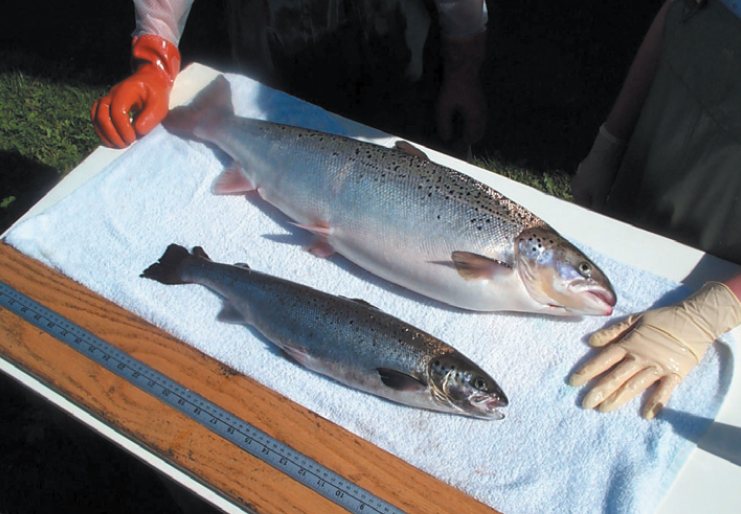
\includegraphics[width=\linewidth]{images/salmon}
\caption{Comparación del crecimiento de un salmón silvestre y un salmón transgénico con incremento en la expresión de la GH(Hormona del Crecimiento)\cite{berkowitz1994transgenic, ledford2013transgenic}}
\label{salmon}
\end{figure}

\subsection{Mascotas Transgénicas}
    
    La transfección permite la obtención de mascotas con características deseables comercialmente que, sin embargo, no se encuentren en estado natural. Estos han creado un nuevo nicho de mercado con un enorme potencial de crecimiento. 
    
    Un ejemplo muy interesante de mascotas transgénicas es el de los peces transgénicos. Inicialmente, Gong y colaboradores en la Universidad de Singapur, modificaron "peces cebra" (\textit{Danio rerio}) para expresar las proteínas fluorescentes GFP (proteína verde fluorescente), YFP (proteína amarillo fluorescente) y RFP (proteína rojo fluorescente) que actúan en asociación con el gen \textit{mylz2}, produciendo diferentes peces de distintos colores fluorescentes. En 2003, la Universidad de Singapur realizó un trato con Yorktown Technologies, que comenzó a comercializarlos como mascotas bajo el nombre comercial de "GloFish" (luego de una evaluación de su posible impacto ambiental y alimenticio llevado a cabo por la FDA)\cite{food2003fda}. Además de estos, existen "peces Medaka" (\textit{Oryzias latipes}) fluorescentes, creados por investigadores de la Universidad de Taiwan y comercializados en dicho país \cite{gong2003development, espinoza2012reproduccion, scotto2013primera}.
    
\begin{figure}[ht]\centering
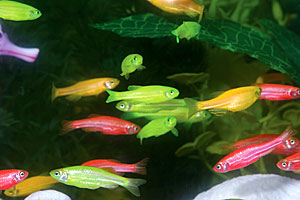
\includegraphics[width=\linewidth]{images/danio}
\caption{`Glofish': \textit{Danio rerio}, ``peces zebra'' que expresan proteínas fluorescentes GFP, YFP y RFP que actúan en asociación con el gen \textit{mylz2} \cite{gong2003development, fox2008fda}}
%\label{fig:danio}
\end{figure}    
    
    Otro caso importante de mascotas genéticamente modificadas es el de los gatos hipoalergénicos, actualmente en desarrollo por la empresa Felix Pets en EEUU. La expresión de la proteína Fel-dI (principal alérgeno, responsable del 90\% de los casos de alergia a gatos en humanos) se puede inhibir, silenciando el gen que la produce mediante la inserción de una secuencia llamada \textit{neo-r} en el primer o segundo intrón del gen\cite{avner2012method, butt2012hypoallergenic}. 
  
\section{Bioética, Opinión Pública y Reglamentación de la Transfección }

Como hemos visto, la transfección tiene múltiples aplicaciones con enorme potencial para mejorar la nutrición y la salud a nivel global. Pese a esto, existe un debate continuo entre legisladores y en la opinión pública respecto a cuales deberían ser los límites de esta biotecnología. Este debate esta fundamentado tanto en prin debido a que existen múltiples preocupaciones de diversos tipos, tanto justificadas como injustificadas, y a un debate bioético sobre la cuales deberían ser los límites de esta biotecnología \cite{berkowitz1993food, berkowitz1994transgenic, mepham1998use, christiansen2000bioethics, Iredale, Cooley, Rowland, Verhoog2003294, Spink, Jefferson,lassen2006after, Ormandy}.

Existen cuatro principios fundamentales de la bioética: \textit{autonomía}(capacidad de decisión de cada individuo), \textit{beneficencia}(realizar el bien a los demás), \textit{no maleficencia}(no perjudicar a los demás) y \textit{justicia}(buscar la igualdad de derechos)\cite{Cooley, tsai2005bioethical}.

Siguiendo estos principios, resulta importante considerar los métodos de transfección per se, y como afectan el bienestar e integridad de los animales. La mayoría de métodos empleados son invasivos porque requieren de acciones como la obtención de muestra seminal, vasectomía o implantación de embriones. Además, la mayoría de métodos son ineficientes (menos de 1\% en mamíferos y entre 10 y 70\% en peces)  que conlleva el empleo de gran cantidad de animales, y en muchos casos su muerte. En ese sentido, la transfección al afectar la vida animal, evidentemente sin posibilidad de decisión de dichos animales, atenta contra todos los principios mencionados. Sin embargo, es importante considerar que dichas acciones invasivas no son únicas de la transfección, que se está buscando desarrollar métodos menos invasivos, que se está investigando para mejorar la eficiencia de los métodos, y que esta biotecnología busca mejorar en muchos sentidos la calidad de vida del ser humano; argumentos que en conjunto justifican, al menos en el sentido de la intención, la transfección dentro de los principios bioéticos \cite{mepham1998use,christiansen2000bioethics, lassen2006after, niemann2007transgenic, Ormandy}. 

En segundo lugar, es relevante aplicar los principios bioéticos al debate sobre la naturalidad en animales transgénicos. En este sentido, podemos analizar el concepto de \textit{'telos'} planteado por Aristóteles. Este concepto implica la esencia y propósito de la existencia de cada ser vivo. En ese sentido, la mayor parte de organismos modificados mediante la transfección estarían en conflicto con su \textit{'telos'} debido a que su esencia se ha modificado para desvirtuar su propósito\cite{Rollin1998}. Sin embargo, pese a que este argumento es en parte cierto, su aplicación práctica debe considerarse inválida, puesto que la crianza tradicional de animales también modifica esta esencia mediante cruces selectivos y que el carácter 'natural' de los seres vivos no necesariamente implica que su fenotipo pueda considerarse bueno tanto para el animal como para el ambiente\cite{Verhoog2003294, Ormandy}. 

Siguiendo en el sentido de la esencia de los seres vivos, existe la posibilidad de la reproducción de peces transgénicos e incluso de su cruzamiento con individuos no transgénicos de la misma especie o especies cercanas, lo cual podría afectar el balance ecosistémico\cite{espinoza2012reproduccion, oke2013hybridization}. Esto podría evitar empleando métodos que eviten la libre reproducción de organismos trangénicos como su contención o poliploidización en caso de los peces \cite{pandian1998ploidy,wong2008transgenic}.

Otra cuestión importante a considerar, y quizá la más importante para la opinión pública es la de los alimentos transgénicos. En esta cuestión el debate se centra en la seguridad de estos alimentos para el consumo humano y en si se debería permitir que se patenten los alimentos, dejando el control del suministro alimenticio esencialmente en mano de las empresas\cite{berkowitz1994transgenic, Jefferson, ledford2013transgenic}.


%----------------------------------------------------------------------------------------
%	REFERENCE LIST
%----------------------------------------------------------------------------------------

\bibliographystyle{unsrt}
\bibliography{referencias}

%----------------------------------------------------------------------------------------

\end{document}
